%!TEX encoding = UTF-8 Unicode
%%%%%%%%%%%%%%%%%%%%%%% file template.tex %%%
%%%%%%%%%%%%%%%%%%%%%%
%
% This is a general template file for the LaTeX package SVJour3
% for Springer journals.          Springer Heidelberg 2010/09/16
%
% Copy it to a new file with a new name and use it as the basis
% for your article. Delete % signs as needed.
%
% This template includehttps://www.overleaf.com/18909956dygyghmktbjfs a few options for different layouts and
% content for various journals. Please consult a previous issue of
% your journal as needed.
%
%%%%%%%%%%%%%%%%%%%%%%%%%%%%%%%%%%%%%%%%%%%%%%%%%%%%%%%%%%%%%%%%%%%
%
% First comes an example EPS file -- just ignore it and
% proceed on the \documentclass line
% your LaTeX will extract the file if required
\begin{filecontents*}{example.eps}
%!PS-Adobe-3.0 EPSF-3.0
%%BoundingBox: 19 19 221 221https://www.overleaf.com/18909956dygyghmktbjf
%%CreationDate: Mon Sep 29 1997
%%Creator: programmed by hand (JK)
%%EndComments
gsave
newpath
  20 20 moveto
  20 220 lineto
  220 220 lineto
  220 20 lineto
closepath
2 setlinewidth
gsave
  .4 setgray fill
grestore
stroke
grestore
\end{filecontents*}
%
\RequirePackage{fix-cm}
%
%%\documentclass{svjour3}                     % onecolumn (standard format)
%%\documentclass[smallcondensed]{svjour3}     % onecolumn (ditto)
\documentclass[smallextended]{svjour3}       % onecolumn (second format)
%\documentclass[twocolumn]{svjour3}          % twocolumn
%
\smartqed  % flush right qed marks, e.g. at end of proof
%
\usepackage{amsmath,amsfonts,amssymb}
\usepackage[latin1]{inputenc}
\usepackage{graphics} %%
\usepackage{graphicx}
\usepackage{subfigure} 
\usepackage[colorlinks=true, allcolors=blue]{hyperref} 
\usepackage[ngerman,english]{babel} 
\usepackage{lineno}
\usepackage{lscape} 
\usepackage{rotating} 
%%\usepackage{natbib} 
\usepackage{color}
\usepackage{soul}
\usepackage{xcolor,colortbl}
% etc.
%
% please place your own definitions here and don't use \def but
% \newcommand{}{}

\newcommand{\tem}[1]{\textcolor{red}{Teresa Mineo: #1}} %Teresa's comments
\newcommand{\anto}[1]{\textcolor{green}{Antonello: #1}} %
\newcommand{\rob}{\textcolor{orange}} 

%\newcommand{\xmm}{\textit{XMM-Newton}}
%\newcommand{\erosita}{\textit{eROSITA}}
%\newcommand{\athena}{\textit{ATHENA}}
\linenumbers
\usepackage{marvosym}

%
% Insert the name of "your journal" with
% \journalname{myjournal}
%
%%\journal{}

%------------------------------------------------------------------------------
% Code for ORCID iD
%------------------------------------------------------------------------------
\usepackage{tikz,xcolor,hyperref}

% Make Orcid icon
\definecolor{lime}{HTML}{A6CE39}
\DeclareRobustCommand{\orcidicon}{%
	\begin{tikzpicture}
	\draw[lime, fill=lime] (0,0) 
	circle [radius=0.16] 
	node[white] {{\fontfamily{qag}\selectfont \tiny ID}};
	\draw[white, fill=white] (-0.0625,0.095) 
	circle [radius=0.007];
	\end{tikzpicture}
	\hspace{-2mm}
}

\foreach \x in {A, ..., Z}{%
	\expandafter\xdef\csname orcid\x\endcsname{\noexpand\href{https://orcid.org/\csname orcidauthor\x\endcsname}{\noexpand\orcidicon}}
}

% Define the ORCID iD command for each author separately.
\newcommand{\orcidauthorA}{0000-0003-4727-9136}
\newcommand{\orcidauthorB}{0000-0002-4931-8445}
\newcommand{\orcidauthorC}{0000-0001-8722-0361}
\newcommand{\orcidauthorD}{0000-0002-9554-4128}
\newcommand{\orcidauthorE}{0000-0001-9204-9749}

\begin{document}

%\title{A semi-empirical model for soft proton scattering at grazing incidence from X-ray mirrors}
\title{The ASTRI-Horn telescope: evaluation of the diffuse night sky background and comparison with UVscope measurements}

%\thanks{Grants or other notes
%about the article that should go on the front page should be
%placed here. General acknowledgments should be placed at the end of the article.}

%\subtitle{Do you have a subtitle?\\ If so, write it here}

\titlerunning{ASTRI-Horn Bkg}        % if too long for running head

\author{Antonio~Alessio~Compagnino\textsuperscript{\Email}\orcidA{} \and Teresa~Mineo\orcidB{} \and Maria~Concetta~Maccarone\orcidC{} \and Osvaldo~Catalano\orcidD{} \and Domenico~Impiombato\orcidE{}}


%\authorrunning{Short form of author list} % if too long for running head
\authorrunning{A.~Compagnino, T.~Mineo, M.C.~Maccarone, O.~Catalano, D.~Impiombato}
\institute{Alessio~Compagnino \and Teresa~Mineo \and Maria~Concetta~Maccarone \and Osvaldo~Catalano \and Domenico~Impiombato\at
              INAF, Istituto di Astrofisica Spaziale e Fisica Cosmica di Palermo, via U. La Malfa 153, I-90146 Palermo, Italy \\ 
              \Email\texttt{\scriptsize{ :alessio.compagnino@inaf.it}}         
           }

\date{Received: date / Accepted: date}
% The correct dates will be entered by the editor

\maketitle

\begin{abstract}
.....


\keywords{}
% \PACS{PACS code1 \and PACS code2 \and more}
% \subclass{MSC code1 \and MSC code2 \and more}
\end{abstract}

\section{Introduction}
\label{sect:intro}


%\textit{\textcolor{blue}{\hl{Cettina: primo draft }}}

\begin{itemize}
\item
ASTRI-Horn (Cettina)
\item
UVscope (Cettina)
\item
task of the article 
\end{itemize}
\section{ASTRI-Horn telescope} 
The ASTRI-Horn telescope is based on a dual mirror system in Schawrzschild-Couder configuration
with a focal length of 2.15 m and a wide field of view (FoV) of 9.6$^\circ$. 
The primary mirror, 4.3 m diameter, is segmented in 18 hexagonal panels, 
while the secondary mirror, 2.2 m diameter, is a monolitic hemispherical thick glass shell. 
Dedicated measurements  with an optical CCD camera showed that the
point spread function (PSF) has a constant width of a few arcmin
over the whole FoV and that  90\% of the PSF  is containerd in one camera pixel (ref). 

The focal surface camera, has a convex-shaped structure where
photon detection modules (PDMs), that are square flat modules, are symmetrically placed
with angles respect to the telescope axis 
opportunely chosen in order to follow the curvature of the focal plane.
Each PDM, composed of 8$\times$8 side-by-side Silicon photomultipliers (SiPMs), 
is installed on a printed circuit board that hosts the front-end electronics (FEE) composed by
 two application specific integrated circuits (ASIC) for the SiPM signal read out.
 The ASTRI camera FEE electronics \cite{Sottile2016} represents an innovative solution, being based on a custom peak-detector operation mode to acquire the SiPM pulses rather than the sampling technique usually adopted by other Cherenkov telescopes.
This FEE-FPGA manages the the generation of local trigger, a topological one, activated when a given number of contiguous pixels within a PDM presents a signal above a given photo-electron threshold \cite{Sottile2016}.
The back-end electronics (BEE) is the main elaboration unit of the camera which
controls and manages the overall system, including data, and
all ancillaries used to perform operations as
the camera thermal regulation, the voltage distribution management and the time events stamping.
The BEE also provides the functions necessary to process and transmit the event data as 
obtained by the FEE to an external data acquisition 
workstation responsible for receiving and storing the data packets \cite{Sottile2016}.
In order to protect the camera sensors from the external
atmospheric environment, an optical-UV transparent poly methyl methacrylate (PMMA)  window 
is mounted onto the focal surface support structure covering all the PDMs.
This window is modeled with the same radius of curvature of the focal surface \cite{Catalano2018}.
The ASTRI SST-2M camera is also equipped  with a light-tight lid to prevents accidental sunlight 
exposure of the focal surface detectors.
The camera is thermally controlled to keep the working temperature on the focal plane within the range 13-17$^\circ$C
for maintaing a goopd gain stability.

A side emitting Fiber Optics system(FOC) is located  along the PMMA  circumference. It is illuminated by a Light Emitting Diode (LED)  system and used for the on-field relative calibration of the gain.  Its light uniformly illuminates the PDMs units at a controlled intensity.




\section{ASTRI-Horn data reduction and analysis} 
\label{sect:astridata}

\subsection{Gain evaluation}
\label{subs:gain}

A first step of the data analysis chain is the calibration of the camera pixel gains. 
The ASTRI-Horn camera is equipped with a thermal control system to keep the temperature of the focal plane in a defined reange and to monitor it in order to coherently change the voltage applied to the FEE preamplifiers (???) and compensate any following  gain variations. In addition, a dedicated procedure is implemented to improve the level of the gain calibration up to 1\% with an off-line analysis. This method is based on the use of a side emitting fiber optics system (FOC) located along the PMMA window circumference and connected to a controlled intensity diode (LED. It lights almost uniformly the focal plane with an average intensity of a few $p.e.$ per pixel. FOC data are collected periodically during the normal telescope acquisition mode (???).

FOC data used for this paper data analyis are listed in Table~\ref{tab:FOC}; they are relative to a fixed voltage $V_{0}$= 57 V {\tem di che?} and a temperature of 15$^\circ$C {\che vuol dire?}. For these acquisitions HG data are available.

The HG pulse hight distribution for both runs listed in Table~\ref{tab:FOC} is accumulated and, for each pixel, the position of the maximum amplitude of each peak is computed fitting the curve with a multi-Gaussian function. Figure~\ref{fig:FOC} shows the pulse height spectrum relative to one of the camera pixel. The gain is computed comparing the average difference between two consecutive peaks centers, $p.e._{eq}$, with that produced by a reference gain $p.e._{ref}$:

\begin{equation}
Gain_{run ID}\,=\,\frac{p.e._{eq}}{p.e._{ref}}\,Gain_{ref}
\end{equation}

\noindent
where $Gain_{run ID}$ is the gain in the considered run, and $Gain_{ref}$ is the reference one.

\begin{figure*}[ht!!]
\centering
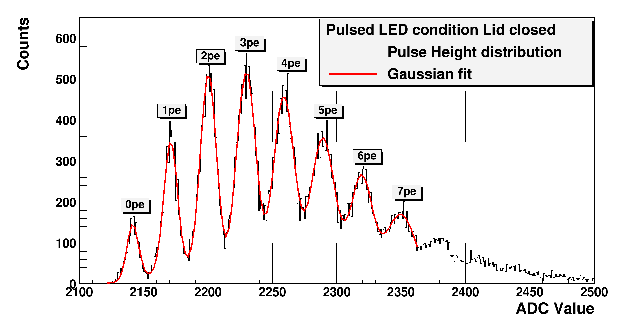
\includegraphics[angle=0, width=12.5cm]{figure/PIXEL60_PDM20_HG_DICEMBRE_2018.eps}
\vspace{0.5cm}
\caption{ Pulse height spectrum for one of the camera pixel during a FOC acquisition (black curve); data are relative to the HG electronics chain. The red curve shows the multiple peaks Gaussian fit.}
\label{fig:FOC}
\end{figure*}

\begin{table*}[htbp!!]
\centering
\caption{Log of FOC data used in the analysis. For these runs HG data are considered. }
\label{tab:FOC}
\begin{tabular}{lccc}
\hline\hline
Run ID & Starting Date &  Expopsure & Number of events \\
               & (year/month/day h:m:s) & (s)   \\
\hline     
1394 & 2018/12/02 20:01:09  &  & 60065     \\
1763 & 2019/03/23 20:01:21  &  & 120123    \\ 
\hline\hline
\end{tabular}
\end{table*}

\subsection{Open sky data} 
\label{subs:skydata}

Background data used for the analysis refer to the period between December 2018 and March 2019 when the telescope was mainly involved in the Crab observation campaign. The list of the considered run ID is reported in Table~\ref{tab:obslog}; runs are split in several files, each containing a maximum of 50000 events, identified with a progressive number.
A selection was applied in order to avoid data affected by technical problems as instability in the PDM signals or fluctuation of the trigger rate. Moreover, intervals with bad atmospheric conditions 
(high humidity, low external temperature, cloudiness) were not considered as well as the periods when UVscope data are not available.

In each detected events we considered only the nine central PDM (11, 12, 13, 18, 19, 20, 25, 26, 27 in Fig.~\ref{fig: camera} ) taking into account the smaller UVscope FOV.  In addition, bad pixels and pixels imaging stars with a magnitude higher than …, coherently with the procedure adopted for UVscope data, are excluded from the analysis. The position of the stars in ASTRI-Horn FOV is computed from the correspondence with UVscope pixels derived from the variance method (Segreto et al 2019). 
The variance method was not used to identify stars because the relative data were not available in December and, for uniformity in the analysis, we decide to not use it either in March.  However, March variance data were used to cross-check the positions obtained from the correspondence with UVscope pixels.

\begin{table}[ht]
\label{tab:astrilog}
\caption{ASTRI-Horn observation log}
\centering
\begin{tabular}{lcccc}
\hline\hline
Run ID & Starting Date & Exposure      & N. of events & pointing \\
               & (year/month/day h:m:s) & (s)  \\
\hline     
%https://www.overleaf.com/project/5e3005eb54e0d8000155a7ff
%\footnote{ Azi$=180°$ EleV. $=70°$}
1429 & 2018/12/05 20:57:37  &   2094     & 31755 & Crab Off    \\
1430 & 2018/12/05 21:54:40  &   909      & 29808 & Fixed AltAzi*    \\
1431 & 2018/12/05 22:22:29  &   3573     & 133190 & Crab     \\ %133188
1432 & 2018/12/05 23:30:12  &   3790     & 450000 & Crab     \\ %449998
1433 & 2018/12/06 01:27:41  &   7638     & 198341 & Crab Off    \\ %198303
1434 & 2018/12/06 03:36:06  &   4499     & 142610 &  Fixed AltAzi$^*$ %142583   \\
1453 & 2018/12/07 20:06:11  &   6016     & 348442 & Crab Off    \\
1454 & 2018/12/07 22:09:16  &   4377     & 226651 &  Crab \\ %226650  \\
1455 & 2018/12/07 23:30:08  &   6243     & 412451 &  Crab \\ %412446    \\
1456 & 2018/12/08 01:24:48  &  8530     & 237318 & Crab Off \\ %  237186 \\
1457 & 2018/12/07 03:50:20  &  3509     & 126295 & Fixed ALtAzi\\ % 126264   \\
1464 & 2018/12/08 20:30:37 &  2255 & 97257 & Crab Off \\ %97251 \\  
1465 & 2018/12/08 21:17:34 &  9624 & 430245 & Crab\\ % 430222\\  
1466 & 2018/12/09 00:07:25 &  3161 & 251442 & Crab \\ %251418  
1467 & 2018/12/08 01:09:44 &  8959 & 243713 & Crab Off \\ %243399
1468 & 2018/12/08 03:40:11 &  1237 & 33168 &  Fixed AltAzi\\ %33126
% **the runs 1488_001 and 1488_002 present an error in TELAPSE keyword 
1472 & 2018/12/09 19:55:03 &  4958 & 185142 &  Crab Off \\ % 185120
1473 & 2018/12/09 21:28:40 &  5549 & 266294 &  Crab\\ %266283
1474 & 2018/12/09 23:19:17 &  3508 & 239982 &  Crab \\ %239954
1475 & 2018/12/10 00:43:51 &  396 & 50989 &  Crab Off \\ %50984
1486 & 2018/12/11 23:02:02 &  1627 & 100948 &  Crab\\ %100947
1487 & 2018/12/11 23:31:48 &  4800 & 259447 &  Crab\\ %259443
1488 & 2018/12/12 01:01:45 &  4638+** & 297577 &  Crab Off\\ %297517
1489 & 2018/12/12 03:02:43 &  1744 & 73285 &  Crab Off \\ %73268
1490 & 2018/12/12 03:34:02 &  5705 & 125218 &  Fixed AltAzi*\\ %124197
1658 & 2019/03/05 18:13:58 &  112 & 1435 & Merak \\  
1659 & 2019/03/05 18:19:26 &  154 & 3149 & Zeta Tauri \\  
1660 & 2019/03/05 18:24:37 &  6224  & 419636 & Crab \\ %419631  
1661 & 2019/03/05 20:10:15 &  168 & 14389 & Zeta Tauri \\  
1662 & 2019/03/05 20:19:59 &  4008 & 198186 & Crab Off \\   
1663 & 2019/03/05 21:29:34 &  2337 & 165264 &  Fixed AltAzi \\  
1670 & 2019/03/06 18:08:27 &  628    &   8191      &  Merak\\
1671 & 2019/03/05 18:21:51 &  126        &   2412   & Zeta Tauri \\
1672 & 2019/03/05 18:25:56 &  5935    &   296073   &  Crab \\ %296046
1673 & 2019/03/05 20:06:58 &  183      &   3272     & Zeta Tauri\\ %3270
1674 & 2019/03/05 20:13:37 &  13812      &    152393 & Crab Off  \\ %152110     \\
%1466 & 2018/12/09 20:47:50 &  1218 & 50000 \\  
\hline\hline
\multicolumn{5}{l}{$^*$ Azi$=180^\circ$ Elev. $=70^\circ$}
\end{tabular}
\end{table}



Background pixels were identified applying the same double cut cleaning procedure used for the Cherenkov shower images. This procedure considers background pixels the ones that have a signal lower than a first threshold $S1$, or , if higher than $S1$, with none of the neighboring pixels with a signal higher that the second threshold $S2$. In our analysis, we adopted the values $S1$=6 and $S2$=12 used by Mineo et al. 2019 instead of higher values adopted for the analysis of Crab events (Lombarbi et al. 2018) to avoid muon signals.

For each event we then accumulated the distribution of the number of $p.e.$ in the background pixels. The curve obtained for the file 1473 of the run ID 000 is plotted in Fig.~\ref{fig:distr} as example. It is a distribution with a Gaussian shape in the central part and with long wings due to residual signals in the positive part and to … ???? in the negative one. 

The central part of the distribution is then fitted with a Gaussian whose $\sigma$ is the measure of the NSB fluctuations that, being a Poissonian signal, is linked to the absolute flux. The RMS values for December 9—10 observation night are plotted in Fig.~\ref{fig:rms} as function of time.

Finally, we plot the resulting values of $\sigma$ for each observing night in Fig.\ref{fig:sigma}  as a function of time. 


\subsection{Closed camera data} 

As explained in Sect.~\ref{sect:intro}, the $\sigma$ of the background distribution is obtained by the sum of the intrinsic noise plus the fluctuations due to the NSB flux level. The first component can be obtained by events acquired with the camera lids closed in absence of light.
Observations used for this analysis are listed in Table~\ref{tab:dark}. In this case, data from LG electronics chain are considered and pulse height spectra for each camera pixels are accumulated adding the contributiond of the two considered observations. These are mainly composed by a single peak, the pedestal, that is fitted with a Gaussian function whose $\sigma$ is the measurement of $\sigma_{dark}$. As example the distribution relative to one of the camera pixel in the run ID 1616 is plotted in Fig.~\ref{fig:dark}).


\begin{figure*}[h!!]
\centering
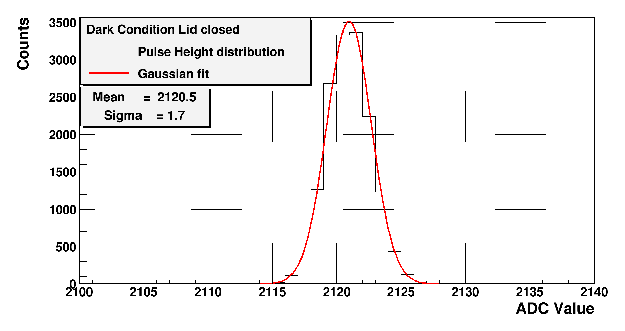
\includegraphics[angle=0, width=12cm]{figure/PIXEL60_PDM20_LG_DICEMBRE_2018.eps}
\vspace{0.5cm}
\caption{ Pulsed height distribution in one of the camera pixel relative to the runs listed in
Table~\ref{table2} (black curve), the the relative fit with a Gaussian (red curve).}
\label{fig:dark}
\end{figure*}
\label{subs:skydata}


\begin{table*}[htbp!!]
\centering
\caption{Log of closed lid observations. For these runs, LG data are considered.}
\label{tab:dark}
\begin{tabular}{lccc}
\hline\hline
Run ID & Starting Date & Exposure     & Number of events \\
               & (year/month/day h:m:s)   \\
\hline     
1380 & 2018/12/01 20:59:18  &       & 15305      \\
1616 & 2019/02/28 12:37:02  &      & 50000     \\
\hline\hline
\end{tabular}
\end{table*}

\newpage
\section{UVscope data reduction and analysis} (Cettina)
\label{sect:uvscopedata}
\section{Results}
\label{sect:results} (Alessio)
\input{conclusion}
\begin{acknowledgements}
This work was conducted in the context of the ASTRI Project, supported by the Italian Ministry of Education, University, and Research (MIUR) with funds specifically assigned to the Italian National Institute of Astrophysics (INAF), and by the Italian Ministry of Economic Development (MISE) within the Astronomia Industriale program. This work has gone through internal review by the ASTRI Project Collaboration.
\end{acknowledgements}
%\addcontentsline{toc}{section}{\numberline{}\bibname}
%%\bibliographystyle{spbasic}      % basic style, author-year citations
%\bibliographystyle{spmpsci}      % mathematics and physical sciences
%\bibliographystyle{spphys}       % APS-like style for physics

%%\begin{small}
\bibliographystyle{plainnat}
%%\bibliography{BIBLIOGRAFIC}
%%\bibliographystyle{unsrtnat}
\bibliography{BIBLIOGRAFIC}

%%\end{small}

%%\clearpage

\end{document}
% end of file template.tex
